\section{Week 8 \& 9, Newns Anderson model}
\subsection{Section 1; The Green function}
\begin{exercise}
Show that the Fourier transform of the uncoupled Green functions are given by 
\begin{equation}\label{eq:uncoupledGreen}
    G_{ij}^0(\omega) = \frac{\delta_{ij}}{\omega - \varepsilon_i + i \eta}
\end{equation}
Where $i,j \in \{k,a\}$ and $\eta$ is a positive infinitesimal.
\end{exercise}

\begin{solution}
The basis independent form the Green function is given by equation 18 in the note on Green functions:
\begin{equation}
   \hat{G}^0(\omega) = \sum_n \frac{\ket{\phi_n} \bra{\phi_n}}{\omega - \varepsilon_n + i \eta}
\end{equation}
We wish to find the uncoupled Greens functions, hence we operate in the basis of the Greens function with the states spanned in $i,j \in \{k,a\}$. Hence each element can be expressed as the matrix element in the following way:
\begin{equation}
     G_{ij}^0(\omega) = \mel{\phi_i}{\hat{G}^0(\omega)}{\phi_j} = \sum_n \frac{\braket{\phi_i}{\phi_n} \braket{\phi_n}{\phi_j}}{\omega - \varepsilon_n + i \eta}
\end{equation}
And as the set of $\phi_m$ constitutes an orthonormal basis the inner products vanish apart from the cases where $i=n=j$, so that
\begin{equation}
    G_{ij}^0(\omega) = \frac{\delta_{ij}}{\omega - \varepsilon_i + i \eta}
\end{equation}
\end{solution}
\subsection{Section 2; Embedding self-energy}
\begin{exercise}
Use equation (4):
\begin{equation}
    \left[(\omega + i \eta)I - H_0 \right]G^0(\omega) = I
    \label{eq:NonInt}
\end{equation}
and (5):
\begin{equation}
        \left[(\omega + i \eta)I - H \right]G(\omega) = I
        \label{eq:WithInt}
\end{equation}
to show that the full Green function, G, fulfills the Dyson equation
\begin{equation}
    G_{aa}(\omega) = G_{aa}^0(\omega) + G_{aa}^0(\omega) \sum_k V_{ak} G_{ak}(\omega)
\end{equation}
\end{exercise}

\begin{solution}
To solve this we first isolate $H_0$ in \eqref{eq:NonInt}
\begin{equation}
    H_0 = -I (G^0)^{-1} + \left[(\omega + i \eta) \right]I
    \label{eq:HIsolated}
\end{equation}
In equation \ref{eq:WithInt} we write $H = H_0 + V$ and plugin equation \ref{eq:HIsolated}
\begin{equation}
    (G^0)^{-1}G(\omega) - V G(\omega) = I
\end{equation}
Now we multiply by $(G^0)$ from the left, and isolate $G(\omega)$ to obtain
\begin{equation}\label{eq:NA210}
    G(\omega) = G^0 V G(\omega) + G^0
\end{equation}
To find $G_{aa}$ we take the inner product with an a bra and ket.
\begin{equation}
    G_{aa} = \mel{a}{G^{0}}{a} + \mel{a}{G^{0}VG}{a}
\end{equation}
As $G^{0}$ is diagonal in $a$ (see equation \ref{eq:uncoupledGreen}) this term reduces trivially, and the remaining term can be found by introducing several "ones" in a spectral representation.
\begin{align}
    G_{aa} &= G^{0}_{aa} + \mel{a}{G^{0}\sum_b\ket{b}\bra{b}V\sum_k\ket{k}\bra{k}G}{a} \\
    &= G^{0}_{aa} + \sum_{b=a}\sum_k\mel{a}{G^{0}\ket{b}\bra{b}V\ket{k}\bra{k}G}{a}\\
    &= G^{0}_{aa} + \sum_k G^{0}_{aa}V_{ak}G_{ka} \label{eq:NA114}
\end{align}
Where it was used that $G^0$ is non interacting so that a has to equal b.
\end{solution}
\begin{exercise}
Write down a similar equation for $G_{ka}(\omega)$ and show that
\begin{equation}
    \sum_{k}V_{ak}G_{ka}(\omega) = \sum G_{kk}^{0}\abs{V_{ak}}^2G_{aa}(\omega)
\end{equation}
and combine the resulting equation in $G_{ak}$ with the result from $G_{aa}$ to obtain
\begin{equation}
    G_{aa}(\omega) = G_{aa}^{0}(\omega) + G_{aa}^{0}(\omega)\Sigma_{aa}(\omega)G_{aa}(\omega) \quad,\quad \Sigma_{aa}(\omega)=\sum_{k}\dfrac{\abs{V_{ak}}^2}{\omega-\varepsilon_k+i\eta}
\end{equation}
\end{exercise}
\begin{solution}
Starting from \eqref{eq:NA210} we may obtain $G_{ka}$ by taking the matrix element $\mel{k}{G}{a}$ with $k\neq a$.
\begin{equation}
    G_{ka} = G_{ka}^{0} + \sum_{k',k''}\mel{k}{G^{0}}{k'}\mel{k'}{V}{k''}\mel{k''}{G}{a}
\end{equation}
as $G^{0}_{ka} = 0$ for all $k\neq a$ and we only consider $k\neq a$ this term is trivially zero. Similarly $k=k'$ following the same argument, removing the $k'$ sum. As $V_{c,d}$ is only non-zero when either $c=a$ and $d\in k$ or $d=a$ and $c\in k$ we must also have that $k''=a$, further removing the $k''$ sum. Hence
\begin{equation}
    G_{ka} = G_{kk}^{0}V_{ka}G_{aa}
\end{equation}
Multiplying by $V_{ak}$ and summing over $k$, and noting that $V_{ak} = V_{ka}^{*}$ we obtain the solution
\begin{equation}\label{eq:NA119}
    \sum_{k}V_{ka}G_{ka} = \sum_{k}G_{kk}^{0}\abs{V_{ka}}^2G_{aa}
\end{equation}
Defining the self energy as
\begin{equation}\label{eq:NA220}
    \Sigma_{aa}(\omega)=\sum_{k}G^{0}_{kk}\abs{V_{ka}}^2=\sum_{k}\dfrac{\abs{V_{ak}}^2}{\omega-\varepsilon_k+i\eta}
\end{equation}
and inserting \eqref{eq:NA119} in \eqref{eq:NA114} we directly obtain the decoupled Dyson-like equation in $G_{aa}$
\begin{equation}
    G_{aa}(\omega) = G_{aa}^{0}(\omega) + G_{aa}^{0}(\omega)\Sigma_{aa}(\omega)G_{aa}(\omega)
\end{equation}
\end{solution}

\subsection{Section 3; Wideband approximation}

\begin{exercise}
If the metal density of states is approximately constatnt in the region of the localising state and the coupling elements $V_{ak}$ varies only little with $k$, the function $\Delta(\omega) =\Delta$ becomes a constant and the real part of the self-energy vanishes. This is known as the wideband limit. \\
Show that the Green function function in this approximation becomes
\begin{equation}
    G_{aa}(\omega) = \frac{1}{\omega - \varepsilon_a+i \Delta/2}
\end{equation}
Calculate and sketch the spectral function $A_a(\omega) = - \mathrm{Im}G_{aa}(\omega)$
\end{exercise}

\begin{solution}
We start of with equation (8) in the project handout and write the self energy as a sum of a real and an imaginary part.
\begin{equation}
    G_{aa}(\omega) = \frac{1}{\omega - \varepsilon_a-(\mathrm{Re}(\Sigma_{aa}(\omega)) + i \mathrm{Im}(\Sigma_{aa}(\omega)))}
\end{equation}
Now we use that the imaginary part is constant, the real part is zero and equation (9) in the project handout, that states that
\begin{equation}
    \mathrm{Im}(\Sigma_{aa}(\omega)) = -\frac{\Delta}{2}
\end{equation}
Upon plugging this in above the result is obtained
\begin{equation}
        G_{aa}(\omega) = \frac{1}{\omega - \varepsilon_a + i \Delta/2}
\end{equation}

To find the imaginary part of this we multiply both the nominator and denominator with the complex conjugate of the denominator to obtain
\begin{equation}
    G_{aa}(\omega) = \frac{\omega - \varepsilon_a - i \Delta/2}{(\omega - \varepsilon_a)^2 + \Delta^2/4}
\end{equation}
So we obtain
\begin{equation}
    A_a(\omega) = - \mathrm{Im}(G_{aa}(\omega)) = \frac{\Delta/2}{(\omega - \varepsilon_a)^2 + \Delta^2/4}
\end{equation}

\begin{figure}[!ht]
    \centering
    \begin{tikzpicture}[scale=1.2]
            \begin{axis}[
                axis lines=middle,
                ticks=none,
                xmin=-1*pi,xmax=4*pi,
                ymin=-0.1,ymax=1.5,
                xlabel={$\omega$},
                ylabel={$A_a(\omega)$},
                domain=-10000:10000,
                restrict y to domain=-1:2,
                enlargelimits=true
                ]
        % parts:
        \addplot[black,domain=-5.1:13 ,unbounded coords=jump,samples=102] {1/((x-2)^2+1)};
        \draw (0,1) -- (-0.3,1) node[left] {$2/\Delta$};
        \draw (2,0) -- (2,-0.05) node[below] {$\omega=\epsilon_a$};
        
        \end{axis}
    \end{tikzpicture}
    \caption{Illustration of the local density of states for the adsorbed molecule, assuming the self energy to be frequency independent.}
    \label{fig:DOSNEWNS}
\end{figure}
This is a lorentzian shape, that is sketched in figure \ref{fig:DOSNEWNS}. As this is the diagonal elements of the spectral function, it describes local density of states.
\end{solution}






\begin{exercise}
Show that the Green function takes the following form in the time domain,
\begin{equation}
    G_{aa}(t) = -i \theta(t)e^{-i(\varepsilon_0-i \Delta/2)t}
    \label{eq:GreenInTime}
\end{equation}
\end{exercise}


\begin{solution}
The easiest way to do this is to Fourier transform \eqref{eq:GreenInTime}, and show that it gives exactly the Green function in the frequency domain given by equation (11) in the problem handout. So we perform the Fourier transform:
\begin{equation}
    G_{aa}(\omega) = \int_{-\infty}^{\infty} -i \theta(t)e^{-i(\varepsilon_0-i \Delta/2)t} e^{i \omega t} \mathrm{d} \omega
\end{equation}
Note that this time there was no reason to include an infinitesimal imaginary part in the Fourier transform to make it converge, as this is handled by the $i \Delta$. \\
The heavyside function means that the fourier transform only runs from 0 to infinity, so the integral is just
\begin{equation}
    G_{aa}(\omega) = \int_{0}^{\infty} -i e^{-i(\varepsilon_0-i \Delta/2 - \omega)t}  \mathrm{d} \omega = \frac{i}{-i(\varepsilon_0-i \Delta/2 - \omega)} = \frac{1}{\omega - \varepsilon_0  + i \Delta/2 }
\end{equation}
Alternatively this may be obtained by starting from the definition of the Greens function, but with an energy correction to the single particle energies such that $\hat{H}_0\ket{N+1,i} = (\varepsilon_0) + \varepsilon_i + i\Delta/2\ket{N+1,i}$ so that
\begin{equation}
        G_{aa}(t) = -i\theta(t)\mathrm{e}^{i\varepsilon_0 t}\left(\mel{N}{c_a(t)\mathrm{e}^{-i\hat{H}_0 t}c^{\dagger}_a(0)}{N} + \mel{N}{c^{\dagger}_a(t)\mathrm{e}^{i\hat{H}_0 t}c_a(0)}{N}\right)
\end{equation}
remembering that the two terms correspond to the electron and hole, respectively, propagating from time $t=0$ to $t$. Focusing on the electron and the cases of $\varepsilon_i < \varepsilon_f$ and $\varepsilon_i > \varepsilon_f$ separately, we see that the first and second term, respectively, equals zero. The remaining terms have the same sign so that regardless of $\varepsilon_i$ it takes the form:
\begin{equation}
    G_{aa}(t) =  -i\theta(t)\mathrm{e}^{-i(\varepsilon_i+i\Delta/2)t}
\end{equation}
With this result we see that $\abs{G_{aa}(t)}^2$ correspond to the probability of the electron (hole for $\varepsilon_i < \varepsilon_f$) inserted at time $t=0$ is still in the same orbital at time $t$. Before introducing the energy correction $i\Delta/2$ the state would be unchanged as it is non-interacting. Now it decays, corresponding to an inverse life time.
\end{solution}

\subsection{Section 4; Discrete approximation}
\begin{exercise}
Assume that $\Delta(\omega)$ can be represented as a delta function located at $<\varepsilon_k>$ and use a drawing to show that $G_{aa}(\omega)$ can have two distinct poles in this case.
\end{exercise}
\begin{solution}
Using the Kramer-Kronig relations we have that
\begin{equation}
    \Gamma(\omega) = \dfrac{P}{2\pi}\int\dfrac{\delta(\omega'-\omega_k)}{\omega-\omega'}\mathrm{d}\omega' = \dfrac{P}{2\pi} \dfrac{1}{\omega - \omega_k} \propto \dfrac{1}{\omega - \omega_k}
\end{equation}
where $\omega_k = <\varepsilon_k>$ and $P$ is the Cauchy principal value. Looking at $G_{aa}(\omega)$ we have that
\begin{equation}
    G_{aa}(\omega) = \dfrac{1}{\omega - \varepsilon_a - \Gamma(\omega) - i\Delta/2}
\end{equation}
Hence it is clear that we have poles at:
\begin{equation}
    \omega - \varepsilon_a - \Gamma(\omega) = 0
\end{equation}
which is a second order polynomial in $\omega$ with two distinct roots when $(\omega_k + \varepsilon_a)^2 - 2P \geq 0$. This may be illustrated by plotting the straight line $(\omega - \varepsilon_a)$ against $\Gamma(\omega)$ as done in figure \ref{fig:discreteapp}. An alternative approach is to interpret the delta function behaviour as collapsing the sum in \eqref{eq:NA220} so that
\begin{equation}
    \Sigma_{aa}(\omega)= \sum_{k}\dfrac{\abs{V_{ak}}^2}{\omega-\varepsilon_k+i\eta} \approx \dfrac{\abs{V_{ak}}^2}{\omega - <\varepsilon_k> + i\eta}
\end{equation}
Hence the imaginary part of $\Sigma_{aa}$ resembles a delta function in the $\eta \rightarrow 0$ at $\omega = <\varepsilon_k>$.
\begin{figure}
    \centering
    \begin{tikzpicture}[scale=1]
        \begin{axis}[
                axis lines=middle,
                ticks=none,
                xmin=-3,xmax=7,
                x label style={at={(current axis.right of origin)},anchor=north},
                xlabel={$\omega$},
                domain=-10000:10000,
                restrict y to domain=-4:5,
                enlargelimits=true
                ]
            % parts:
            \addplot[black,domain=-3:1.999,samples=102, unbounded coords=jump] {1.7/(x-2)};
            \addplot[black,domain=2.001:10,samples=102, unbounded coords=jump] {1.7/(x-2)};
            \addplot[black,domain=-3:10,samples=102] {(x-1)};
            \draw (1,0.1) -- (1,-0.3) node[below] {$\varepsilon_a$};
            \draw (2,0.1) -- (2,-0.3) node[below] {$\omega_k$};
            \node at (7,5) {$\omega - \varepsilon_a$};
            \node at (2.1,5) {$\Gamma(\omega)$};
            \draw (2.9,1.89) circle (0.2);
            \draw (0.1,-0.9) circle (0.2);
        \end{axis}
    \end{tikzpicture}
    \caption{Schematic illustration of the two poles of $G_{aa}$ for the discrete approximation. The poles are highlighted with circles and are found as the intersection of the two curves $\Gamma(\omega)$ and $\omega-\varepsilon_a$.}
    \label{fig:discreteapp}
\end{figure}
\end{solution}
\subsection{Section 5; Semi-elliptic band}
\begin{exercise}
Show that the imaginary part of the complex function
\begin{equation}\label{eq:semi-ellipse}
    f(z) = a(z/b - \sqrt{[(z+i\eta)/b]^2 - 1})
\end{equation}
regarded as a function of $x = \mathrm{Re}\{z\}$ describes a semi-ellipse of height $a$ and width $2b$. Argue that if $\Delta(\omega)$ us a semi-ellipse of height $a$, width $2b$, $\Gamma(\omega)$ can be obtained from the real part of $f(z)$ and is given by
\begin{equation}\label{eq:Gamma-SE}
    \Gamma(\omega) = \dfrac{a}{2}\left(\omega/b - \theta(\abs{\omega}-b)\mathrm{sign}(\omega)\sqrt{(\omega/b)^2-1} \right)
\end{equation}
\end{exercise}
\begin{solution}
In this case the self energy is represented by \eqref{eq:semi-ellipse}, and thus the imaginary, $\Delta/2$, and real, $\Gamma$, parts are obtained from $f(z)$. Regarding $z$ as real and remembering that we have to work in the limit of $\eta \rightarrow 0$ the only way $f(z)$ can have an imaginary part is when the argument of the square-root is negative. This can readily be seen to be when $\abs{z/b}^2 < 1$. Analysing the imaginary part: $\mathrm{Im}\{f(z)\} \neq 0$ we have that
\begin{equation}
    \mathrm{Im}\{f(z)\} = \begin{cases} -a\sqrt{1 - (z/b)^2} &, z^2 \leq b^2 \\ 0 &, z^2 > b^2 \end{cases}
\end{equation}
This can be recognised as a semi-ellipse of height $a$, width $2b$, and centered at $z = 0$. This means that if $\Delta(\omega)$ is a semi-ellipse with the aforementioned parameters, $\Gamma(\omega)$ can be obtained by the real part of $f(z)/2$ (remembering that $\Delta/2 = \mathrm{Im}\{\Sigma\}$. The real part may be obtained in a similar fashion by analysing the two cases separately
\begin{equation}
    \mathrm{Re}\{f(z)\} = \begin{cases} az/b &, z^2 \leq b^2 \\ az/b - \sqrt{(z/b)^2-1} &, z^2 > b^2 \end{cases}
\end{equation}
Letting $z \rightarrow \omega$ we may alternatively write both functions as continuous functions (in contrast to the piece-wise formulation) through the use of the heavy-side function at $\theta(\abs{\omega} - b)$. Hence
\begin{align}\label{eq:semi_gamma}
    \Gamma(\omega) &= \dfrac{a}{2}\left(\omega/b - \theta(\abs{\omega}-b)\sqrt{(\omega/b)^2-1}\right) \\
    \Delta(\omega) &= -\theta(\abs{\omega}-b)a\sqrt{(\omega/b)^2-1} \label{eq:semi_delta}
\end{align}

\end{solution}

\begin{exercise}
Assume that $\Delta(\omega)$ is a semi-ellipse of width 2, height $a$ and centered at $\omega = 0$. Sketch $\Delta(\omega)$ and $\Gamma(\omega)$. Draw also the straight line $\omega-\varepsilon_a$ for $\epsilon_a = 0$, as well as the spectral function:
\begin{equation}\label{eq:semi_spec}
    A_a(\omega) = -\dfrac{1}{2\pi} \dfrac{\Delta(\omega)}{(\omega - \varepsilon_a -\Gamma(\omega))^2 + (\Delta(\omega)/2)^2}
\end{equation}
in the two cases where $a \gg 1$ (strong coupling) and $a \ll 1$ (weak coupling). Discuss the results and compare with the wide band and discrete approximations.
\end{exercise}
\begin{solution}
The semi-elliptic model allows for a continuous transition from the extremely de-localised bands (wideband approximation), e.g. s-bands, to the extremely localised bands (Discrete model), e.g. molecules and atoms. As a consequence we may be able to model the most pronounced features of e.g. the d-bands which lies somewhere in between the discrete and wideband approximation. We see that for strong coupling, $a \gg 1$ we have two poles in the Greens function as in the case of the discrete approximation, where as for weak coupling $a \ll 1$ the spectral density resembles the shape from the wideband approximation. Hence we are able to model the transition from two distinct poles in the Greens function to one, or none. Figure \ref{fig:semi-ellipse} sketches $\Gamma$, $\Delta$, $A_a$ and $\omega - \varepsilon_a$ making use of equations (\ref{eq:semi_gamma}), (\ref{eq:semi_delta}), and (\ref{eq:semi_spec}), for strong and weak coupling.

\begin{figure}
\begin{minipage}{0.49\textwidth}
    \centering
        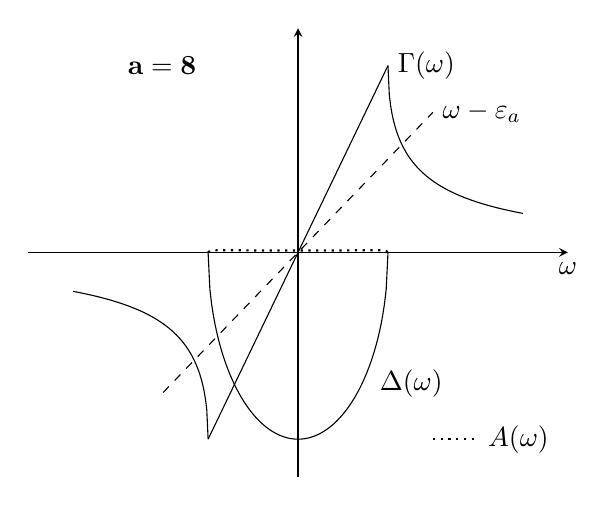
\begin{tikzpicture}[scale=1]
            \begin{axis}[
                    axis lines=middle,
                    ticks=none,
                    xmin=-5,xmax=5,
                    x label style={at={(current axis.right of origin)},anchor=north},
                    xlabel={$\omega$},
                    domain=-2:2,
                    restrict y to domain=-10:10,
                    enlargelimits=true
                    ]
                % Gamma
                \addplot[black,domain=-2:2,samples=102, unbounded coords=jump] {8*0.25*x};
                \addplot[black,domain=-5:-2,samples=102, unbounded coords=jump] {8*(0.25*x + 0.5*sqrt(0.25*x^2-1))};
                \addplot[black,domain=2:5,samples=102, unbounded coords=jump] {8*(0.25*x - 0.5*sqrt(0.25*x^2-1))};
                
                % Delta
                \addplot[black,domain=-2:2,samples=102, unbounded coords=jump] {-8*0.5*sqrt(1-0.25*x^2)};
                
                % omega-epsilon_a
                \addplot[dashed,black,domain=-3:3,samples=102, unbounded coords=jump] {x)};
                
                % Spectral function 
                \addplot[thick,dotted,black,domain=-2:2,samples=102, unbounded coords=jump] {(1/(2*3.14))*(8*0.5*sqrt(1-0.25*x^2))/((x-(8*0.5*0.5*x))^2 + (-8*0.5*sqrt(1-0.25*x^2))^2)};
                
                % LEGEND
                \draw[dotted,thick] (3,-4) -- (4,-4) node[right] {$A(\omega)$};
                \node[right] at (3,3) {$\omega - \varepsilon_a$};
                \node[right] at (2,4) {$\Gamma(\omega)$};
                \node[right] at (1.6,-2.8) {$\Delta(\omega)$};
                \node[right] at (-4,4) {$\mathbf{a = 8}$};
            \end{axis}
    \end{tikzpicture}
\end{minipage}
\begin{minipage}{0.49\textwidth}
\centering
    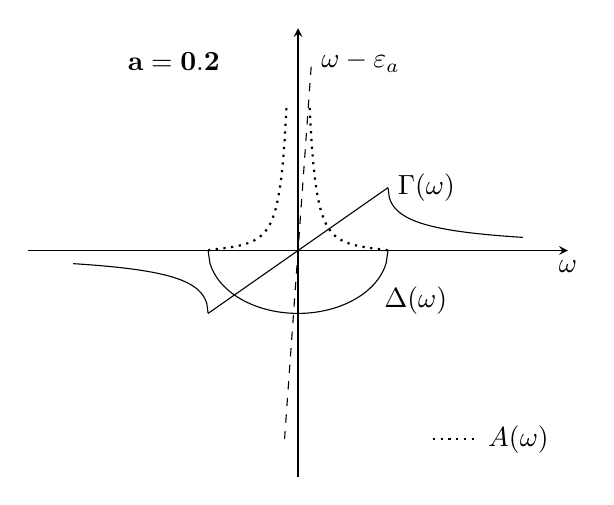
\begin{tikzpicture}[scale=1]
        \begin{axis}[
                axis lines=middle,
                ticks=none,
                xmin=-5,xmax=5,
                x label style={at={(current axis.right of origin)},anchor=north},
                xlabel={$\omega$},
                domain=-2:2,
                restrict y to domain=-0.3:0.3,
                enlargelimits=true
                ]
            % parts:
            % Gamma
            \addplot[black,domain=-2:2,samples=102, unbounded coords=jump] {0.2*0.25*x}; %|x| < b
            \addplot[black,domain=-5:-2,samples=102, unbounded coords=jump] {0.2*(0.25*x + 0.5*sqrt(0.25*x^2-1))}; % x < b
            \addplot[black,domain=2:5,samples=102, unbounded coords=jump] {0.2*(0.25*x - 0.5*sqrt(0.25*x^2-1))}; % x > b
            
            % Delta
            \addplot[black,domain=-2:2,samples=102, unbounded coords=jump] {-0.2*0.5*sqrt(1-0.25*x^2)};
            
            % omega - epsilon_a
            \addplot[dashed,black,domain=-0.3:0.3,samples=102, unbounded coords=jump] {x)};
            
            % Spectral function 
            \addplot[thick,dotted,black,domain=-2:2,samples=102, unbounded coords=jump] {(1/(2*3.14))*(0.2*0.5*sqrt(1-0.25*x^2))/((x-(0.2*0.5*0.5*x))^2 + (-0.2*0.5*sqrt(1-0.25*x^2))^2)};
            
            % LEGEND
            \draw[dotted,thick] (3,-0.3) -- (4,-0.3) node[right] {$A(\omega)$};
            \node[right] at (0.3,0.3) {$\omega - \varepsilon_a$};
            \node[right] at (2,0.1) {$\Gamma(\omega)$};
            \node[right] at (1.7,-0.08) {$\Delta(\omega)$};
            \node[right] at (-4,0.3) {$\mathbf{a = 0.2}$};
        \end{axis}
    \end{tikzpicture}
\end{minipage}
    \caption{Schematic illustration of the semi-elliptic model for strong ($a=8$) and weak ($a=0.2$) coupling, with $\varepsilon_a = 0$ and $b=2$.}
    \label{fig:semi-ellipse}
\end{figure}
\end{solution}
